\documentclass[a4paper]{article}
\usepackage[14pt]{extsizes} % для того чтобы задать нестандартный 14-ый размер шрифта
\usepackage[left=1.5cm,right=1.5cm,top=2cm,bottom=2cm]{geometry}
\usepackage{multirow}
\usepackage{parallel}
\usepackage {graphicx}
\usepackage{multicol}
\usepackage[utf8x]{inputenc} % указать кодировку русского текста
\usepackage[russian]{babel} % указать, что язык текста - русский
\usepackage{fancyhdr}
\pagestyle{fancy}
\usepackage{graphicx}
\graphicspath{{pictures/}}
\DeclareGraphicsExtensions{.pdf,.png,.jpg, .jpeg}
\usepackage{tocloft}
\usepackage{wrapfig}
\usepackage{tikz}

\usepackage{enumitem}
\setlist[enumerate,itemize]{leftmargin=0pt,itemindent=2.7em}
\renewcommand{\cftsecleader}{\cftdotfill{\cftdotsep}}
\begin{document} 
\large
\noindent \textbf{Лабораторная работа 4.1.2: Моделирование оптических приборов и определение их увеличения}\\
\\
\normalsize
\textbf{М.Шлапак}\\
\line(1,0){18cm}\\
\\
\footnotesize
\textit{Изучены модели астрономической трубы Кеплера, земной трубы Галилея, микроскопа; определены их увеличения}\\
\\
\textit{\textbf{Ключевые слова:} зрительная труба, микроскоп, оптические приборы, линзы, юстировка, оптические системы}\\
\fancyhead[L] {Моделирование оптических приборов, М.Шлапак}

\begin{multicols}{2}

\begin{enumerate}
\small
\item \textbf{Введение}\\ 
\noindent 
Одним из важных начальных навыков работы с оптическими приборами является умение правильно их юстировать и центрировать на оптической скамье. В данной работе, помимо этого, также были измерены фокусные расстояния набора линз и смоделированы трубы Кеплера и Галилея, а также микроскоп и измерено их увеличение различными способами.\\
\item \textbf{Экспериментальная установка}
\begin{center}
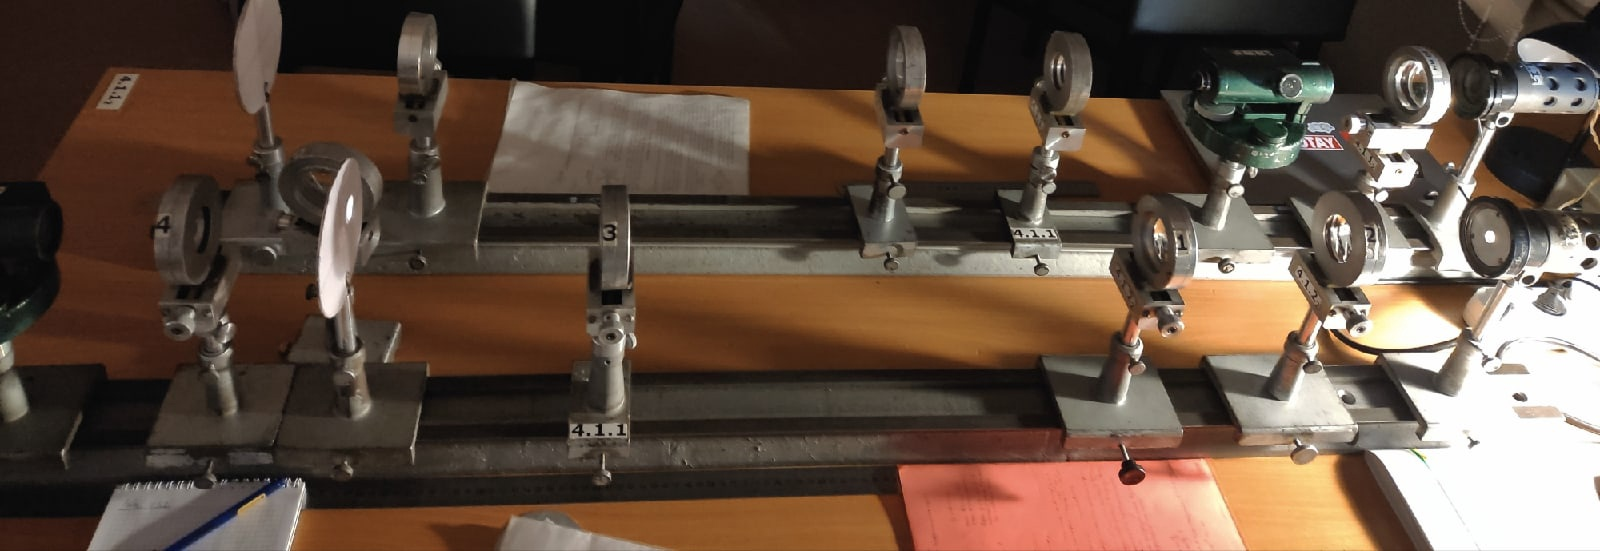
\includegraphics[width=9cm]{exp1}\\
\textit{Экспериментальная установка}
\end{center}

состоит из набора линз, осветителя, оптической скамьи, экрана, зрительной трубы и миллиметровой сетки в качестве рассматриваемого предмета\\
\item \textbf{Результаты эксперимента}\\
В данной работе экспериментально определялись фокусные расстояния набора линз, а также увеличения зрительных труб и микроскопов различными способами. Один из важнейших этапов, от которых зависела точность измерений - центрировка элементов оптической системы.\\
\begin{enumerate}
\item \textbf{Центрировка элементов оптической системы}\\
1) Отберём из всего набора линз собирающие. Для этого, держа линзу в одной руке, получим на ладони другой руки изображение лампочки и оценим на глаз фокусные расстояния. Те из линз, которые не дадут действительного изображения, будут рассеивающими.\\
В результате получаем 4 собирающих и 1 рассеивающую линзы. \\
Запишем номера линз и их примерное фокусное расстояние, измеренное на глаз:\\
\\
\begin{tabular}{|l|l|l|l|l|l|}
\hline
номер линзы & 1 & 2 & 3 & 4 & 5\\
\hline
f, см & 7,5 & 12 & 23 & 40,5 & 11,5\\
\hline
\end{tabular}\\
\\
Соберём и отцентрируем установку таким образом, чтобы главная оптическая ось проходила через центры всех оптических элементов.
\item \textbf{Определение фокусных расстояний тонких линз с помощью зрительной трубы}\\
2)Для определения фокусных расстояний линз настроим зрительную трубу на бесконечность. \\
Соберем установку для определения фокусных расстояний собирающих линз с помощью зрительной трубы:\\
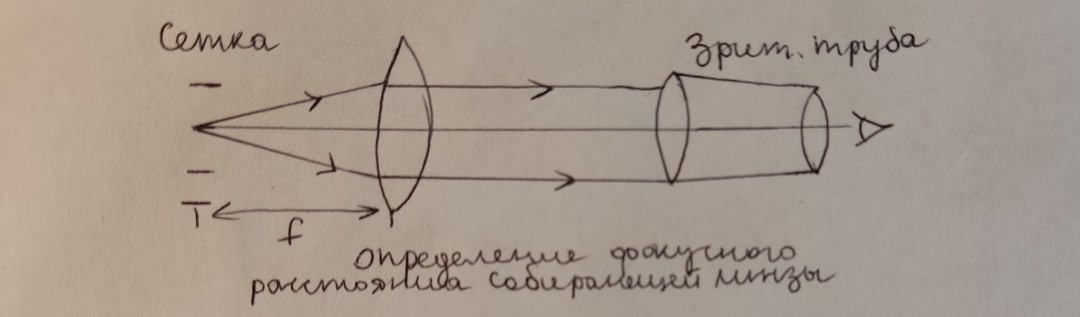
\includegraphics[width=9cm]{exp3}\\
Передвигая линзу вдоль скамьи, получим в окуляре зрительной трубы изображение предмета - миллиметровой сетки. \\
Измерим таким образом фокусные расстояния 4 собирающих линз:\\
\\
\begin{tabular}{|l|l|l|l|l|}
\hline
номер линзы & 1 & 2 & 3 & 4\\
\hline
f, см & 7,5 & 10,7 & 19 & 27,6\\
\hline
\end{tabular}\\
\\
3) Для определения фокусного расстояния тонкой рассеивающей линзы сначала получим на экране увеличенное изображение сетки при помощи одной короткофокусной собирающей линзы. Измерим расстояние $a_0$ между линзой и экраном: $a_0 = 29,0 \pm 0,1$ см. \\
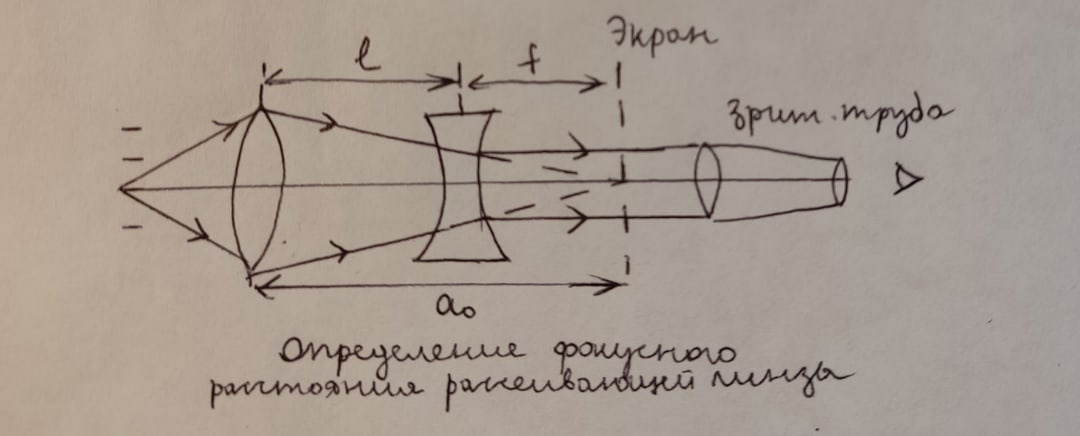
\includegraphics[width=9cm]{exp4}\\
Разместим сразу за экраном трубу, настроенную на бесконечность. Далее вместо экрана поставим рассеивающую линзу. После центрировки, перемещая рассеивающую линзу, найдём в окуляре зрительной трубы резкое изображение сетки. Измерив расстояние между линзами $l$, рассчитаем фокусное расстояние рассеивающей линзы: 
$$f = l - a_0$$
В нашем случае:\\
\begin{center}
\begin{tabular}{|l|l|}
\hline
 $a_0$, см & $29,0 \pm 0,1$ \\
 \hline
 $l$, см & $20,6 \pm 0,1$\\
 \hline
 $f$, см & $-8,4 \pm 0,2$ \\
 \hline
\end{tabular}
\end{center}
\item \textbf{Телескоп Кеплера}\\
4) Отберём из имеющегося набора две собирающие линзы для создания модели зрительной трубы Кеплера с увеличением 2 - 3.\\ 
В качестве коллиматора возьмем линзу 3 с фокусным расстоянием $19$ см. Соберём модель телескопа:\\
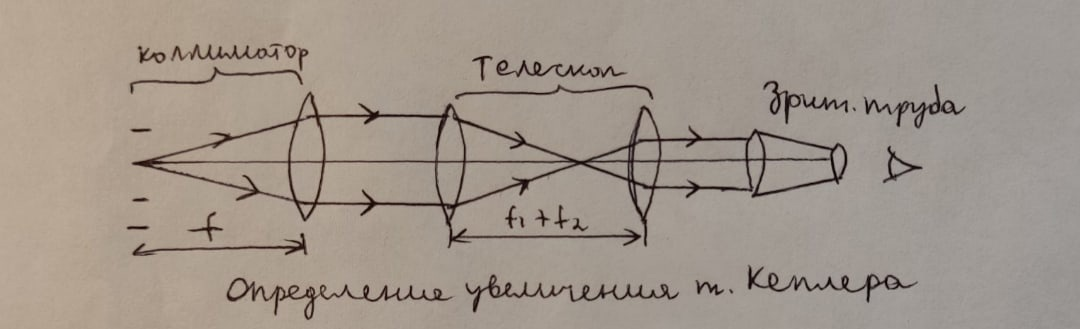
\includegraphics[width=9cm]{exp5}\\
В качестве объектива и окуляра возьмём, соответственно, линзы 4 и 1. Сравним расстояние между объективом и окуляром с суммой фокусных расстояний:
\begin{center}
\begin{tabular}{|l|l|}
\hline
$a$, см & $36,9 \pm 0,1$\\
\hline
$f_1 + f_2$, см & $35,1 \pm 0,2$\\
\hline
\end{tabular}
\end{center}
Для последующих расчётов увеличения телескопа определим размер изображения $h_1$ одного миллиметра шкалы осветителя в делениях окулярной шкалы зрительной трубы:
$$h_1 = k \tg \alpha_1 \approx k\alpha_1$$
,где $k$ - некоторый коэффициент, характеризующий увеличение зрительной трубы, $\alpha_1$ - угловой размер изображения миллиметрового деления шкалы осветителя, наблюдаемого через коллиматор.
$$h_1 = 1 \; \textit{деление}$$ 
- толщина линии миллиметровки\\
5) Рассчитаем увеличение исследуемой модели телескопа через отношение передних фокусных расстояний линз $f_1$ и $f_2$
$$N_{T1} = - \frac{f_1}{f_2}$$
$$N_{T1} \approx - (3,68 \pm 0,05)$$
6) Определим увеличение телескопа через отношение углов, под которыми объект виден через телескоп и без него.\\
$$N_{T2} = - \frac{\alpha_2}{\alpha_1} = - \frac{h_2}{h_1}$$
, где учтено различие знаков углов лучей на входе и выходе из трубы Кеплера.\\
В нашем эксперименте $h_2 = 3,5 \; \textit{деления}$
$$N_{T2} \approx - (3,5 \pm 0,5)$$
7) Определим увеличение телескопа, сравнив диаметр оправы его объектива и диаметр изображения этой оправы в окуляре. \\
$$N_{T3} = - \frac{D_1}{D_2}$$
, где $D_1$ - диаметр объектива, $D_2$ - диаметр его изображения.\\
В нашем случае $D_1 = 3,7 \pm 0,1$ см, $D_2 = 1,0 \pm 0,1$ см.\\
$$N_{T3} \approx - (3,7 \pm 0,4)$$


\item \textbf{Труба Галилея}\\
8) Соберем модель трубы Галилея, поставив в модели трубы Кеплера вместо собирающей окулярной линзы рассеивающую линзу на расстоянии от объектива, равном разности модулей фокусных расстояний объектива и окуляра. Проведем измерения, аналогичные тем, которые были проделаны для телескопа Кеплера.\\
9) Рассчитаем увеличение исследуемой модели телескопа через отношение передних фокусных расстояний линз $f_1$ и $f_2$
$$N_{T1} = - \frac{f_1}{f_2}$$
В нашем случае $f_2 = - 8,4$ см - фокусное расстояние рассеивающей линзы.\\
$$N_{T1} \approx 3,29 \pm 0,05$$
10) Определим увеличение телескопа через отношение углов, под которыми объект виден через телескоп и без него.\\
$$N_{T2} =  \frac{\alpha_2}{\alpha_1} =  \frac{h_2}{h_1}$$
В нашем эксперименте $h_2 = 3,0 \; \textit{деления}$
$$N_{T2} \approx  3,0 \pm 0,5$$
\begin{center}
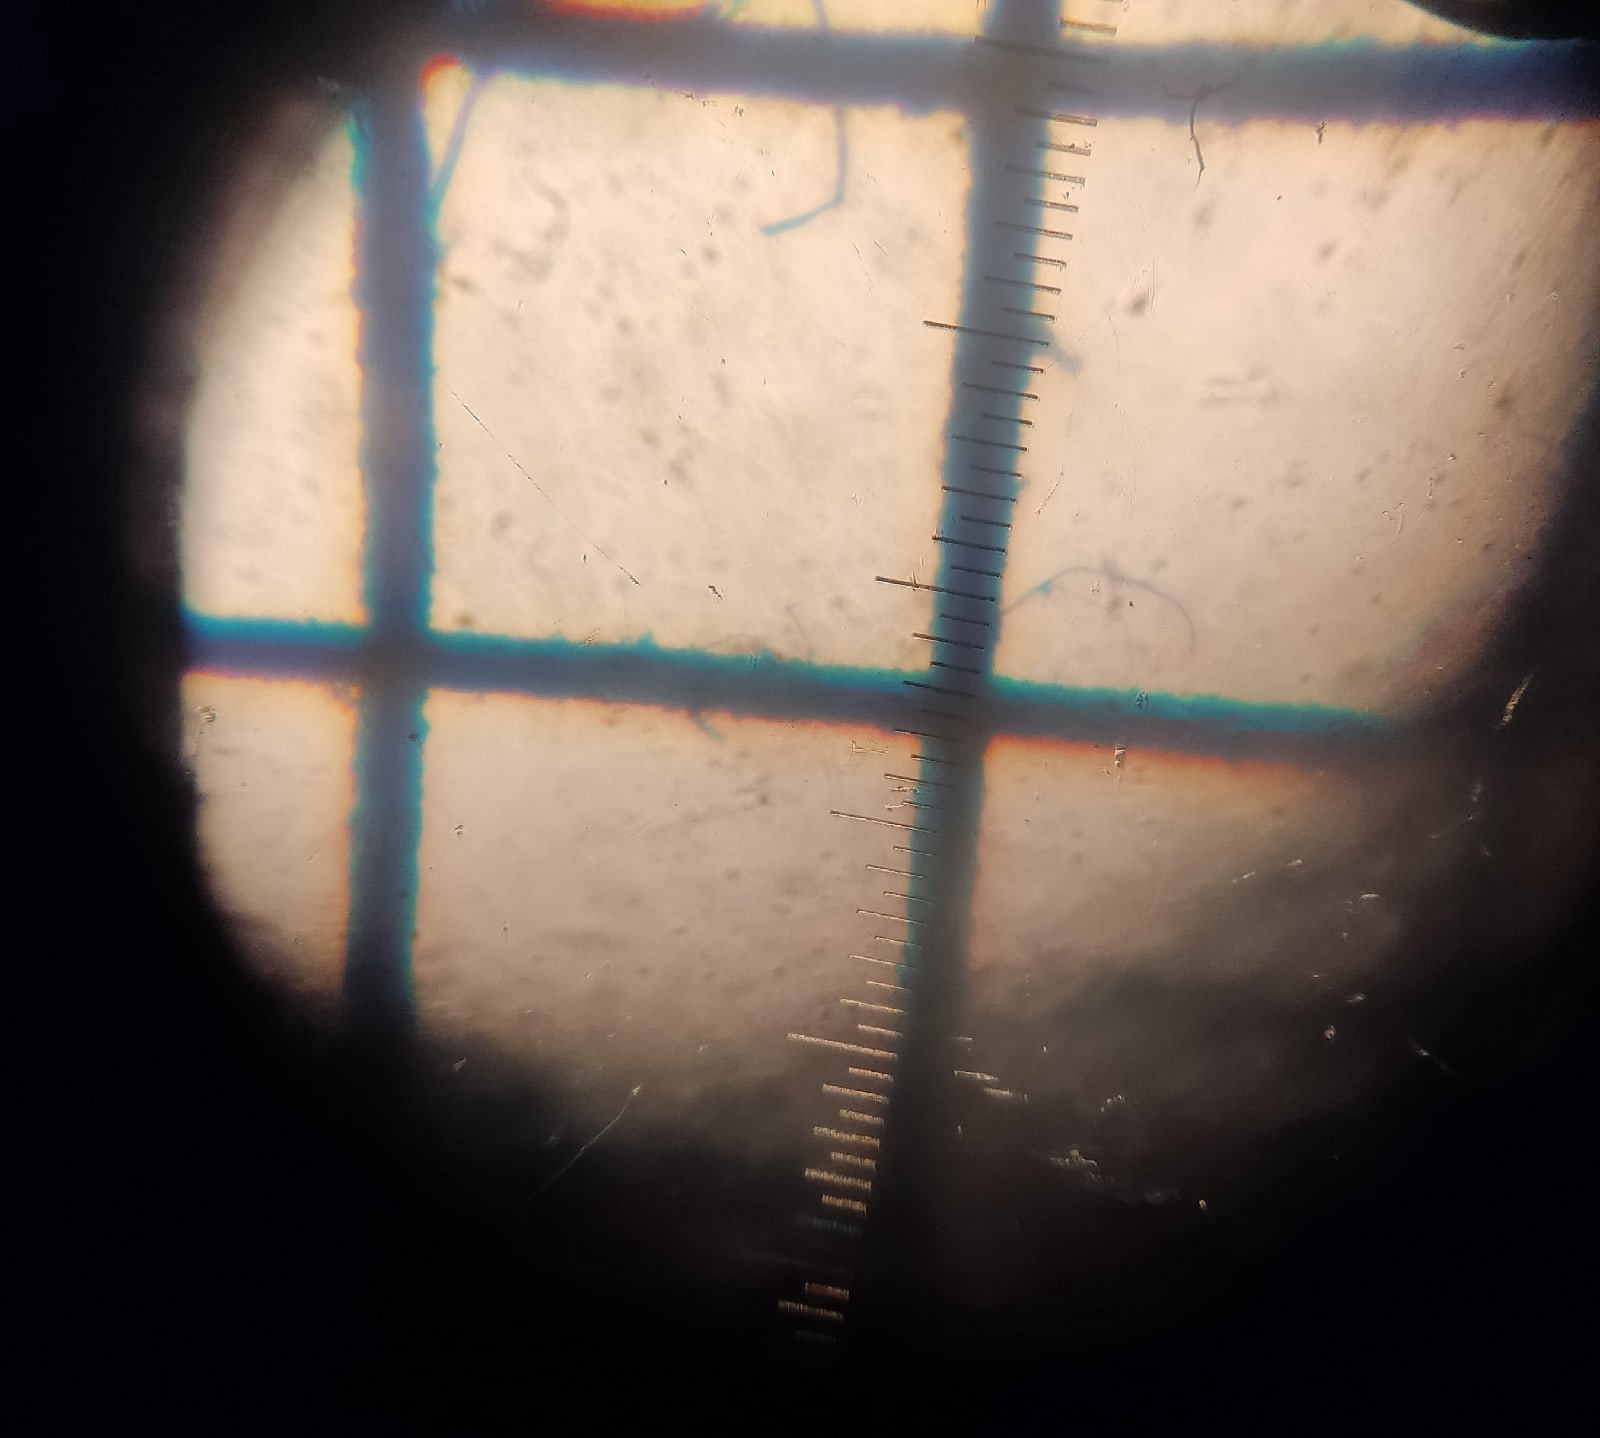
\includegraphics[width=9cm]{exp2}\\
\textit{Определение размера изображения }
\end{center}
\item \textbf{Микроскоп}\\
11) Для создания микроскопа с увеличением $N_{M} = 5$ отберем самые короткофокусные собирающие линзы из набора - линзы 1 и 2.\\
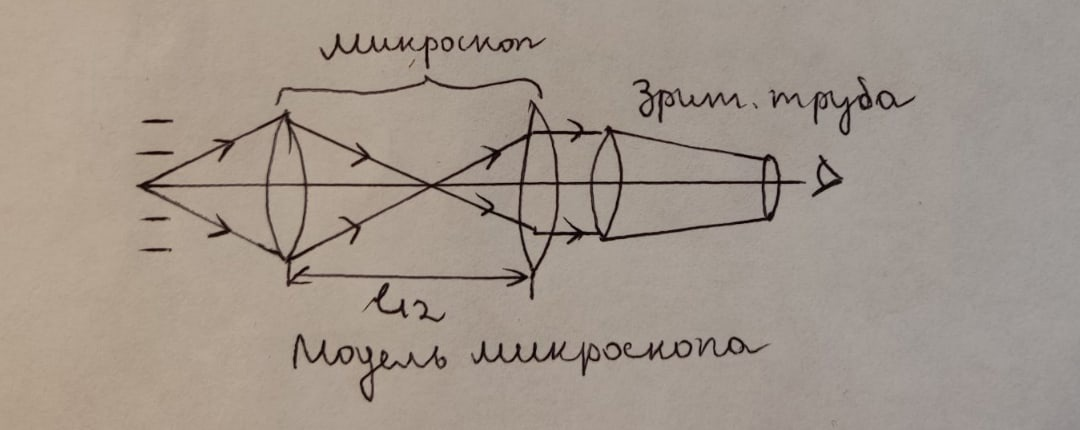
\includegraphics[width=9cm]{exp6}\\
Рассчитаем необходимый оптический интервал $\Delta$ и длину тубуса $l_{12}$ по формулам:
$$M_{M} = N_1N_2$$
$$N_1 = - \frac{\Delta}{f_1}$$
$$N_2 = - \frac{L}{f_2}$$
$$\Delta = l_{12} - f_1 - f_2$$
, где $N_1$ и $N_2$ - увеличения объектива и окуляра, $f_1$ и $f_2$ - фокусные расстояния линз, $L = 25$ см - расстояние наилучшего зрения.\\
$$l_{12} = 34,25 \pm 0,04$$
12) Расположим объектив и окуляр на соответствующем расстоянии $l_{12}$ друг от друга и закрепим рейтеры. Соберём модель микроскопа.\\
15) Для экспериментального определения увеличения микроскопа измерим величину изображения $h_2$ клетки на миллиметровке, зараннее измерив эту же величину без оптической системы $h_1$:\\
$h_1 = 9 \; \textit{делений}$, $h_2 = 35 \; \textit{делений}$\\
13) Используя результат измерений $h_1$ с коллиматорной линзой, фокус которой мы знаем, расчитаем увеличение микроскопа по формуле
$$N_{M} = - \frac{h_2L}{h_1f}$$
$$N_{M} \approx 5,1 \pm 0,3$$
Экспериментальное значение неплохо сходится с теоретическим расчётом.\\
 \end{enumerate}
 \item \textbf{Заключение}
 В данной работе были экспериментально определены фокусные расстояния набора линз двумя способами - грубо и точнее, а также найдено увеличение труб Кеплера (3 способами), Галилея (2 способами) и микроскопа (1 способом). Результаты эксперимента приведены в графиках ниже.\\
 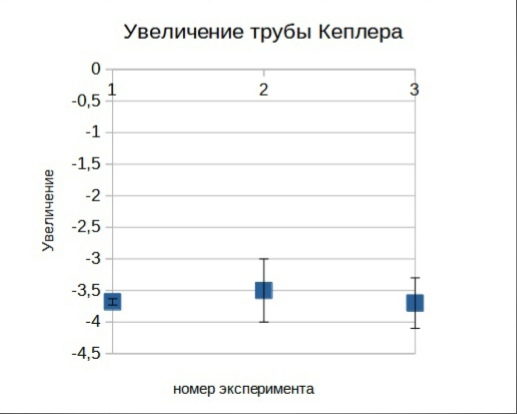
\includegraphics[width = 9cm]{g1}\\
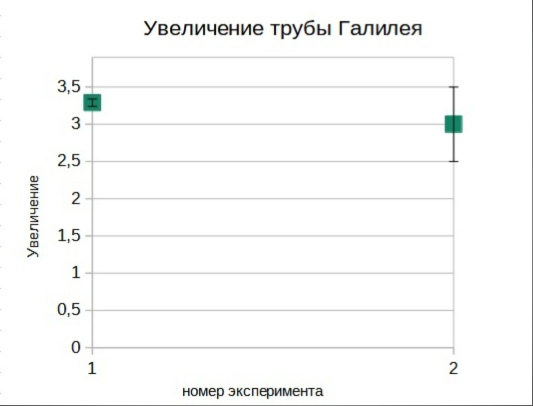
\includegraphics[width = 8cm]{g4}\\
 \end{enumerate}
 \textit{1. Общий курс физики. Оптика, Д.В.Сивухин}\\
\textit{2. Лабораторный практикум по общей физике. Оптика, А.В. Максимычев}\\
\end{multicols}
\end{document}